\documentclass[border=6pt]{standalone}
\usepackage{lmodern}
\usepackage{tikz}
\usepackage{amsmath,amssymb}
\usetikzlibrary{arrows.meta,positioning,calc}

\definecolor{kmblue}{HTML}{003874}
\definecolor{kmgold}{HTML}{BA9224}
\definecolor{rtpurple}{HTML}{7E22CE}
\definecolor{rtgreen}{HTML}{15803D}
\definecolor{rtred}{HTML}{DC2626}
\definecolor{axgray}{HTML}{94A3B8}
\definecolor{dkgray}{HTML}{334155}

\begin{document}
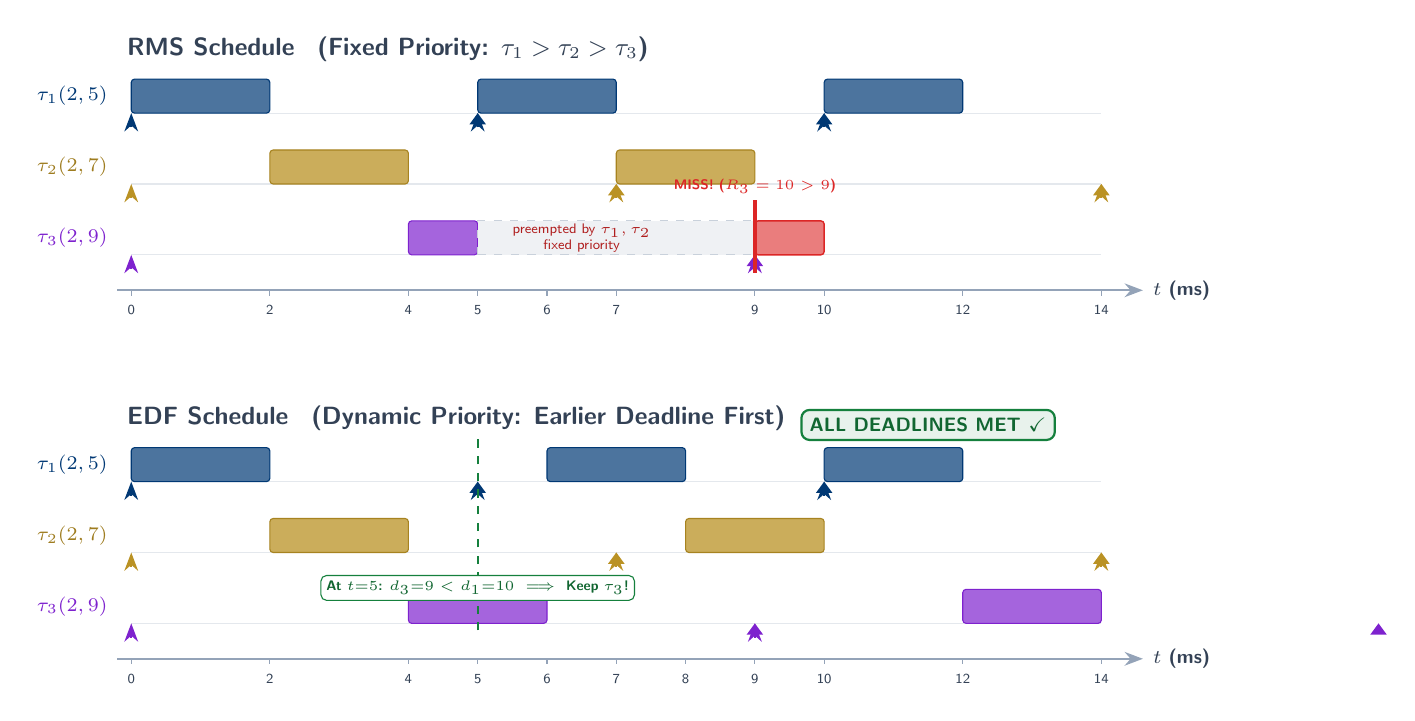
\begin{tikzpicture}[>=Stealth,font=\sffamily,x=0.88cm,y=0.9cm]

  \def\h{0.48} % bar height

  % =====================================================================
  % TOP PANEL — RMS (Fixed Priority: tau1 > tau2 > tau3)
  % =====================================================================
  \def\yA{4.8} % tau1 row
  \def\yB{3.8} % tau2 row
  \def\yC{2.8} % tau3 row

  \node[dkgray,font=\sffamily\small\bfseries,anchor=west] at (-0.2, 5.7)
        {RMS Schedule \enspace (\emph{Fixed Priority:} $\tau_1 > \tau_2 > \tau_3$)};

  % Time axis RMS
  \draw[axgray,line width=0.8pt,->] (-0.2, 2.3) -- (14.6, 2.3)
        node[right,font=\sffamily\scriptsize\bfseries,dkgray] {$t$ (ms)};
  \foreach \t in {0,2,4,5,6,7,9,10,12,14} {
    \draw[axgray] (\t,2.3) -- (\t,2.22)
          node[below,font=\sffamily\tiny,dkgray] {\t};
  }

  % Row guides
  \draw[axgray!25,line width=0.4pt] (0,\yA) -- (14,\yA);
  \draw[axgray!25,line width=0.4pt] (0,\yB) -- (14,\yB);
  \draw[axgray!25,line width=0.4pt] (0,\yC) -- (14,\yC);

  % Task labels
  \node[anchor=east,kmblue,font=\sffamily\scriptsize\bfseries] at (-0.2,\yA+0.5*\h) {$\tau_1(2,5)$};
  \node[anchor=east,kmgold!85!black,font=\sffamily\scriptsize\bfseries] at (-0.2,\yB+0.5*\h) {$\tau_2(2,7)$};
  \node[anchor=east,rtpurple,font=\sffamily\scriptsize\bfseries] at (-0.2,\yC+0.5*\h) {$\tau_3(2,9)$};

  % --- RMS Executions ---
  % tau1: [0,2], [5,7], [10,12]
  \foreach \s/\e in {0/2, 5/7, 10/12} {
    \fill[kmblue!70,rounded corners=1.2pt] (\s,\yA) rectangle (\e,\yA+\h);
    \draw[kmblue,line width=0.4pt,rounded corners=1.2pt] (\s,\yA) rectangle (\e,\yA+\h);
  }

  % tau2: [2,4], [7,9]
  \foreach \s/\e in {2/4, 7/9} {
    \fill[kmgold!75,rounded corners=1.2pt] (\s,\yB) rectangle (\e,\yB+\h);
    \draw[kmgold!90!black,line width=0.4pt,rounded corners=1.2pt] (\s,\yB) rectangle (\e,\yB+\h);
  }

  % tau3: [4,5] (preempted at 5), [9,10] OVERDUE
  \fill[rtpurple!70,rounded corners=1.2pt] (4,\yC) rectangle (5,\yC+\h);
  \draw[rtpurple,line width=0.4pt,rounded corners=1.2pt] (4,\yC) rectangle (5,\yC+\h);
  
  % Preemption gap [5,9] for tau3
  \fill[axgray!15] (5,\yC) rectangle (9,\yC+\h);
  \draw[axgray!50,dashed,line width=0.4pt] (5,\yC) rectangle (9,\yC+\h);

  % Overdue execution [9,10]
  \fill[rtred!60,rounded corners=1.2pt] (9,\yC) rectangle (10,\yC+\h);
  \draw[rtred,line width=0.5pt,rounded corners=1.2pt] (9,\yC) rectangle (10,\yC+\h);

  % Releases (arrows)
  \foreach \t in {0,5,10} \draw[kmblue,line width=0.8pt,->] (\t,\yA-0.2) -- (\t,\yA);
  \foreach \t in {0,7,14} \draw[kmgold,line width=0.8pt,->] (\t,\yB-0.2) -- (\t,\yB);
  \foreach \t in {0,9}    \draw[rtpurple,line width=0.8pt,->] (\t,\yC-0.2) -- (\t,\yC);

  % Deadlines (triangles)
  \foreach \t in {5,10}  \fill[kmblue] (\t,\yA) -- (\t-0.12,\yA-0.16) -- (\t+0.12,\yA-0.16) -- cycle;
  \foreach \t in {7,14}  \fill[kmgold] (\t,\yB) -- (\t-0.12,\yB-0.16) -- (\t+0.12,\yB-0.16) -- cycle;
  \fill[rtpurple] (9,\yC) -- (8.88,\yC-0.16) -- (9.12,\yC-0.16) -- cycle;

  % RMS Deadline Miss Marker
  \draw[rtred,line width=1.2pt] (9,\yC-0.25) -- (9,\yC+\h+0.3);
  \node[rtred,font=\sffamily\bfseries\tiny,above=0pt] at (9,\yC+\h+0.25) {MISS! ($R_3=10>9$)};

  % Preemption callout
  \node[rtred!80!black,font=\sffamily\tiny,align=center] at (6.5, \yC+0.5*\h)
        {preempted by $\tau_1,\tau_2$\\fixed priority};

  % =====================================================================
  % BOTTOM PANEL — EDF (Dynamic Priority based on Absolute Deadline)
  % =====================================================================
  \def\yD{-0.4} % tau1 row
  \def\yE{-1.4} % tau2 row
  \def\yF{-2.4} % tau3 row

  \node[dkgray,font=\sffamily\small\bfseries,anchor=west] at (-0.2, 0.5)
        {EDF Schedule \enspace (\emph{Dynamic Priority:} Earlier Deadline First)};

  % Time axis EDF
  \draw[axgray,line width=0.8pt,->] (-0.2, -2.9) -- (14.6, -2.9)
        node[right,font=\sffamily\scriptsize\bfseries,dkgray] {$t$ (ms)};
  \foreach \t in {0,2,4,5,6,7,8,9,10,12,14} {
    \draw[axgray] (\t,-2.9) -- (\t,-2.98)
          node[below,font=\sffamily\tiny,dkgray] {\t};
  }

  % Row guides
  \draw[axgray!25,line width=0.4pt] (0,\yD) -- (14,\yD);
  \draw[axgray!25,line width=0.4pt] (0,\yE) -- (14,\yE);
  \draw[axgray!25,line width=0.4pt] (0,\yF) -- (14,\yF);

  % Task labels
  \node[anchor=east,kmblue,font=\sffamily\scriptsize\bfseries] at (-0.2,\yD+0.5*\h) {$\tau_1(2,5)$};
  \node[anchor=east,kmgold!85!black,font=\sffamily\scriptsize\bfseries] at (-0.2,\yE+0.5*\h) {$\tau_2(2,7)$};
  \node[anchor=east,rtpurple,font=\sffamily\scriptsize\bfseries] at (-0.2,\yF+0.5*\h) {$\tau_3(2,9)$};

  % --- EDF Executions ---
  % tau1: [0,2], [6,8], [10,12]
  \foreach \s/\e in {0/2, 6/8, 10/12} {
    \fill[kmblue!70,rounded corners=1.2pt] (\s,\yD) rectangle (\e,\yD+\h);
    \draw[kmblue,line width=0.4pt,rounded corners=1.2pt] (\s,\yD) rectangle (\e,\yD+\h);
  }

  % tau2: [2,4], [8,10]
  \foreach \s/\e in {2/4, 8/10} {
    \fill[kmgold!75,rounded corners=1.2pt] (\s,\yE) rectangle (\e,\yE+\h);
    \draw[kmgold!90!black,line width=0.4pt,rounded corners=1.2pt] (\s,\yE) rectangle (\e,\yE+\h);
  }

  % tau3: [4,6] (NO preemption at t=5 because d3=9 < d1=10!), [12,14]
  \foreach \s/\e in {4/6, 12/14} {
    \fill[rtpurple!70,rounded corners=1.2pt] (\s,\yF) rectangle (\e,\yF+\h);
    \draw[rtpurple,line width=0.4pt,rounded corners=1.2pt] (\s,\yF) rectangle (\e,\yF+\h);
  }

  % Releases (arrows)
  \foreach \t in {0,5,10} \draw[kmblue,line width=0.8pt,->] (\t,\yD-0.2) -- (\t,\yD);
  \foreach \t in {0,7,14} \draw[kmgold,line width=0.8pt,->] (\t,\yE-0.2) -- (\t,\yE);
  \foreach \t in {0,9}    \draw[rtpurple,line width=0.8pt,->] (\t,\yF-0.2) -- (\t,\yF);

  % Deadlines (triangles)
  \foreach \t in {5,10}  \fill[kmblue] (\t,\yD) -- (\t-0.12,\yD-0.16) -- (\t+0.12,\yD-0.16) -- cycle;
  \foreach \t in {7,14}  \fill[kmgold] (\t,\yE) -- (\t-0.12,\yE-0.16) -- (\t+0.12,\yE-0.16) -- cycle;
  \foreach \t in {9,18}  \fill[rtpurple] (\t,\yF) -- (\t-0.12,\yF-0.16) -- (\t+0.12,\yF-0.16) -- cycle;

  % EDF Priority decision callout at t=5
  \draw[rtgreen,line width=0.8pt,dashed] (5,-2.5) -- (5,0.2);
  \node[draw=rtgreen,fill=white,rounded corners=2pt,inner sep=2pt,font=\sffamily\tiny\bfseries,text=rtgreen!80!black]
        at (5, -1.9) {At $t{=}5$: $d_3{=}9 < d_1{=}10 \implies$ Keep $\tau_3$!};

  % All Met badge
  \node[draw=rtgreen,fill=rtgreen!10,text=rtgreen!80!black,rounded corners=3pt,line width=0.8pt,font=\sffamily\bfseries\scriptsize,inner sep=3pt]
        at (11.5, 0.4) {ALL DEADLINES MET \checkmark};

\end{tikzpicture}
\end{document}
